\documentclass[tikz]{standalone}
\usepackage{tikz}
\usepackage{anyfontsize}
\usetikzlibrary{arrows.meta, angles, quotes, decorations.markings}

\begin{document}
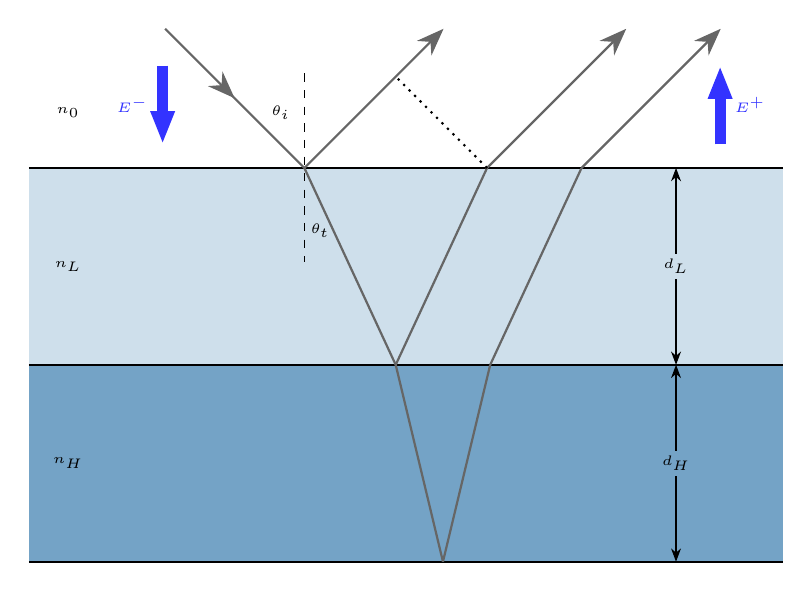
\begin{tikzpicture}[
    every node/.style={font=\tiny},
    % Estilo para el haz incidente (Flecha Gris Gruesa)
    rayoIncidente/.style={
        thick, black!60,
        postaction={decorate, decoration={markings,
            mark=at position 0.5 with {\arrow[black!60]{Stealth[scale=1.5]}}}
        }
    },
    % Estilo para los haces emergentes (Gris Grueso)
    rayoEmergente/.style={
        thick, black!60, -{Stealth[scale=1.5]}
    },
    % Estilo para las flechas de campo E
    flechaE/.style={
        thick, -{Stealth[scale=1.5]}
    },
    flechaE_institucional/.style={
        line width=4pt,
        blue!80,
        -{Triangle[length=12pt, width=8pt]}
    }
]
    % --- CONFIGURACIÓN DE PARÁMETROS ---
    \def\dist{2.5}       
    \def\posX{3.5}       
    \def\despl{1.16}     
    \def\desplExtra{0.6} 
    \def\largoV{1.2}     
    
    % --- DEFINICIÓN DE COLORES ---
    \definecolor{miAzulCapainferior}{RGB}{116, 163, 198} % #74A3C6
    \colorlet{azulCapaL}{miAzulCapainferior!35!white} 
    \colorlet{azulCapaH}{miAzulCapainferior}
    
    % Posiciones calculadas
    \pgfmathsetmacro{\posXcota}{\posX + 2*\desplExtra + 2*\despl + 1.2} 
    \pgfmathsetmacro{\posXEp}{\posX + 2*\desplExtra + 2*\despl + 1.76}
    \pgfmathsetmacro{\anchoTotal}{\posXEp + 0.8} 
    
    % 1. Definición de puntos clave
    \coordinate (I1) at (\posX, 0);                 
    \coordinate (I2) at (\posX + \despl, -\dist);   
    \coordinate (I3) at (\posX + 2*\despl, 0);
    \coordinate (I4) at (\posX + \despl + \desplExtra, -2*\dist); 
    \coordinate (I5) at (\posX + \despl + 2*\desplExtra, -\dist); 
    \coordinate (I6) at (\posX + 2*\desplExtra + 2*\despl, 0);
    
    % Puntos auxiliares
    \coordinate (InPt) at ([shift={(I1)}]135:2.5);
    \coordinate (ReflPt) at ([shift={(I1)}]45:2.5);
    \coordinate (OutPt) at ([shift={(I3)}]45:2.5);
    \coordinate (OutFinalPt) at ([shift={(I6)}]45:2.5);

    % --- FONDOS DE LAS CAPAS ---
    \fill[azulCapaL] (0, 0) rectangle (\anchoTotal, -\dist);      
    \fill[azulCapaH] (0, -\dist) rectangle (\anchoTotal, -2*\dist); 

    % 2. INTERCARAS
    \draw[thick] (0, 0) -- (\anchoTotal, 0);
    \draw[thick] (0, -\dist) -- (\anchoTotal, -\dist);
    \draw[thick] (0, -2*\dist) -- (\anchoTotal, -2*\dist);

    % 3. Normal (Solo en la primera intercara)
    \draw[dashed] (\posX, \largoV) -- (\posX, -\largoV); 

    % 4. Rayos externos (Grises y Gruesos)
    \draw[rayoIncidente] (InPt) -- (I1); 
    \draw[rayoEmergente] (I1) -- (ReflPt);  
    \draw[rayoEmergente] (I3) -- (OutPt);   
    \draw[rayoEmergente] (I6) -- (OutFinalPt);    

    % 5. Trayectoria interna (Gris y Grueso)
    \draw[thick, black!60] (I1) -- (I2);    
    \draw[thick, black!60] (I2) -- (I3);
    \draw[thick, black!60] (I2) -- (I4); 
    \draw[thick, black!60] (I4) -- (I5); 
    \draw[thick, black!60] (I5) -- (I6); 

    % 6. Construcción punteada (Gris y Grueso)
    \draw[dotted, thick] (I3) -- (\posX + \despl, 1.16);

    % 7. Etiquetas de ángulos 
    \node at (\posX-0.3, 0.7) {$\theta_i$};
    \node at (\posX + 0.5 * \despl - 0.38, -0.8) {$\theta_t$};

    % 8. COTAS 'd_L' y 'd_H'
    \draw[{Stealth}-{Stealth}] (\posXcota, 0) -- (\posXcota, -\dist)
        node[midway, fill=azulCapaL, inner sep=2pt] {$d_L$};
    \draw[{Stealth}-{Stealth}] (\posXcota, -\dist) -- (\posXcota, -2*\dist)
        node[midway, fill=azulCapaH, inner sep=2pt] {$d_H$};

    % 9. ÍNDICES n
    \node at (0.5, 0.7) {$n_0$}; 
    \node[fill=azulCapaL, inner sep=2pt] at (0.5, -0.5*\dist) {$n_L$};
    \node[fill=azulCapaH, inner sep=2pt] at (0.5, -1.5*\dist) {$n_H$};

    % 10. CAMPOS E
    
    \draw[flechaE_institucional] (1.7, 1.3) -- (1.7, 0.3) node[midway, left] {$E^-$};
    \draw[flechaE_institucional] (\posXEp, 0.3) -- (\posXEp, 1.3) node[midway, right] {$E^+$};

\end{tikzpicture}
\end{document}